\documentclass{beamer}

\usepackage[utf8]{inputenc}
\usecolortheme{beaver}
\usepackage{caption}
\usepackage{subcaption}
\usepackage{mathtools}
\usepackage{todonotes}
\usepackage{amsmath}
\usepackage{bm}
\usepackage{listings}
\usepackage{ragged2e}
\usepackage{titlecaps}
\usepackage{fancyvrb}
\usepackage{minted}
\usepackage{xcolor}
\definecolor{LightGray}{gray}{0.9}

\def\ci{\perp\!\!\!\!\!\perp}

\newtheorem{proposition}{Proposition}
\Addlcwords{for a is but and with of in as the etc on to if}

\newcommand\github{\includegraphics[height=3ex]{imgs/github.png}}
\newcommand\email{\includegraphics[height=3ex]{imgs/email.png}}

\setbeamertemplate{section in toc}{\inserttocsectionnumber.~\inserttocsection}
\usetheme{Boadilla}
\makeatletter
\setbeamertemplate{footline}{%
    \leavevmode%
    \hbox{%
        \begin{beamercolorbox}[wd=.3\paperwidth,ht=2.25ex,dp=1ex,center]{author in head/foot}%
            \usebeamerfont{author in head/foot}\insertshortauthor\expandafter\beamer@ifempty\expandafter{\beamer@shortinstitute}{}{~~(\insertshortinstitute)}
        \end{beamercolorbox}%
        \begin{beamercolorbox}[wd=.55\paperwidth,ht=2.25ex,dp=1ex,center]{title in head/foot}%
            \usebeamerfont{title in head/foot}\insertshorttitle
        \end{beamercolorbox}%
        \begin{beamercolorbox}[wd=.15\paperwidth,ht=2.25ex,dp=1ex,right]{date in head/foot}%
            \usebeamerfont{date in head/foot}\insertshortdate{}\hspace*{2em}
            \insertframenumber{} / \inserttotalframenumber\hspace*{2ex} 
        \end{beamercolorbox}}%
        \vskip0pt%
    }
\makeatother

\begin{document}

\title[Causal Inference using pgmpy]{Introduction to Casual Inference using pgmpy}
\author{Ankur Ankan}
\institute[]{Postdoctoral Researcher \\ Radboud University, The Netherlands}
\date{}

\maketitle

\begin{frame}{Predictive vs Causal Modelling}
\end{frame}

\begin{frame}{Motivating Examples}
	\begin{itemize}
		\item Finding how variables interact.
		\item Key drivers of an outcome.
		\item Feature Selection
	\end{itemize}
\end{frame}

\begin{frame}{Motivating Examples}
\end{frame}

\begin{frame}{Motivating Examples}
\end{frame}

\begin{frame}{Two Main Framworks}
	Mathematical frameworks for causal inference:
	\vspace{0.5em}
	\begin{itemize}
		\item Potential Outcomes Framework (a.k.a. Rubin's Casual Model)
			\begin{itemize}
				\item Counterfactual statement at the core.
				\item Provides statistical methods for estimating the counterfactual such Propensity Score based methods, Dobly robust estimators, etc.
				% \item Statistically robust methods that can deal with assumption violations.
			\end{itemize}
	\end{itemize}
	\vspace{2em}
	\begin{itemize}
		\item Directed Acyclic Graphs (DAGs) / Structural Equation Models (SEMs)
			\begin{itemize}
				\item Causal diagram, i.e., DAG at the core.
				\item Causal effect estimators can be defined using the DAG.
				\item Modelling assumptions are explicit.
			\end{itemize}
	\end{itemize}
\end{frame}

\begin{frame}{Landscape of Causal Inference Python Packages}
	\begin{columns}
		\begin{column}{0.5 \textwidth}
			\center{\textbf{Potential Outcomes Framework}}
			\begin{itemize}
				\item Collection of estimation methods
					\begin{figure}
						\includegraphics[scale=0.2]{imgs/dowhy.png}
					\end{figure}
				\item Doubly Robust Estimation
					\begin{figure}
						\includegraphics[scale=0.1]{imgs/doubleml.png}
					\end{figure}
				\item Meta Learners: T/S/X-Learners.
					\begin{figure}
						\includegraphics[scale=0.3]{imgs/causalml.png}
					\end{figure}
			\end{itemize}

		\end{column}
		\vrule
		\begin{column}{0.5 \textwidth}
			\center{\textbf{DAG Framework}}
			\begin{itemize}
				\item pgmpy
					\begin{figure}
						\includegraphics[scale=0.2]{imgs/pgmpy.png}
					\end{figure}
				\item casualnex
					\begin{figure}
						\includegraphics[height=2cm, width=3cm, scale=0.2]{imgs/causalnex.png}
					\end{figure}
			\end{itemize}
			\vspace{2em}
		\end{column}
	\end{columns}
\end{frame}

\begin{frame}{A General Workflow in the DAG Framework}
	\begin{figure}
		\centering
		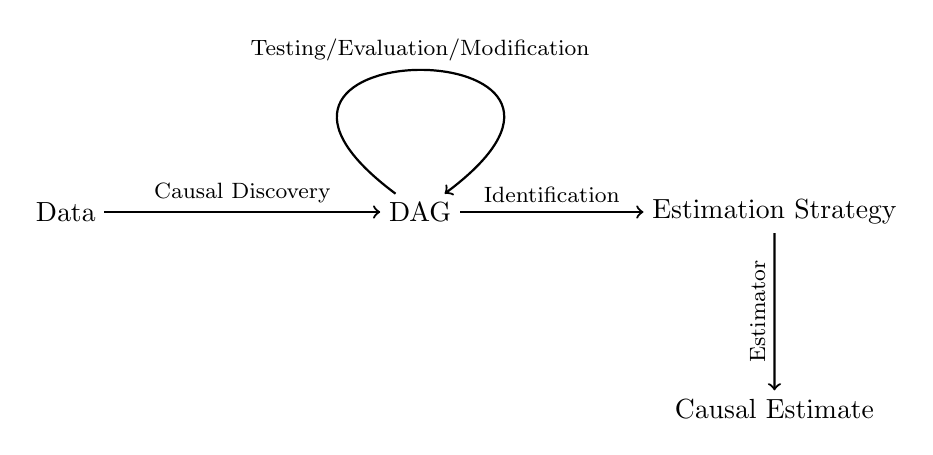
\begin{tikzpicture}[yscale=1, xscale=0.75, inner sep=3pt]
		\tikzstyle{every node}=[align=left]
			\node (data) at (0, 0) {Data};
			\node (dag) at (6, 0) {DAG};
			\node (estimand) at (12, 0) {Estimation Strategy};
			\node (estimation) at (12, -2.5) {Causal Estimate};
	
			\draw[thick, ->] (data) to node[midway, above]{\footnotesize Causal Discovery} (dag);
			\draw[thick, ->] (dag) to node[midway, above] {\footnotesize Identification} (estimand);
			\draw[thick, ->] (estimand) to node[midway, above, rotate=90] {\footnotesize Estimator} (estimation);
			\draw[thick, ->] (dag) [out=150, in=30, looseness=10] to node[midway, above] {\footnotesize Testing/Evaluation/Modification} (dag);
		\end{tikzpicture}
		\label{fig:workflow}
	\end{figure}

	\vspace{1em}

	\center{pgmpy provides functionality to perform each of these steps}

\end{frame}

% \begin{frame}{What does pgmpy provide}
% 	Will show how to perform each of these steps in pgmpy.
% 	\begin{itemize}
% 		\item Provides standardized implementations of commonly used algorithms.
% 		\item Practical methods methods.
% 		\item Extensible.
% 	\end{itemize}
% \end{frame}

\begin{frame}{Causal Discovery}
	\begin{figure}
		\centering
		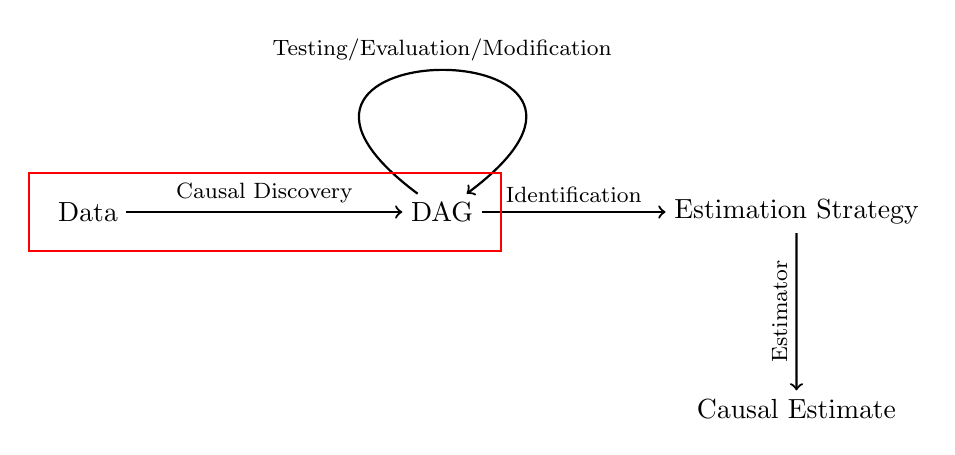
\begin{tikzpicture}[yscale=1, xscale=0.75, inner sep=3pt]
		\tikzstyle{every node}=[align=left]
			\node (data) at (0, 0) {Data};
			\node (dag) at (6, 0) {DAG};
			\node (estimand) at (12, 0) {Estimation Strategy};
			\node (estimation) at (12, -2.5) {Causal Estimate};
	
			\draw[thick, ->] (data) to node[midway, above]{\footnotesize Causal Discovery} (dag);
			\draw[thick, ->] (dag) to node[midway, above] {\footnotesize Identification} (estimand);
			\draw[thick, ->] (estimand) to node[midway, above, rotate=90] {\footnotesize Estimator} (estimation);
			\draw[thick, ->] (dag) [out=150, in=30, looseness=10] to node[midway, above] {\footnotesize Testing/Evaluation/Modification} (dag);

			\draw[draw=red, thick] (-1, -0.5) rectangle (7, 0.5);
		\end{tikzpicture}
		\label{fig:workflow1}
	\end{figure}
	\vspace{1em}
	\center \textbf{Casual Discovery: } Learn the causal DAG from data.
\end{frame}

\begin{frame}{Automated Causal Discovery Algorithms}
	\begin{itemize}
		\item Many automated algorithms with nice asymptotic properties.
			\begin{itemize}
				\item Constraint-based: PC, Fast Causal Inference.
				\item Score-based: Greedy Equivalence Search, Hill-Climb Search.
				\item Optimization-based: NoTears, DAGMA.
			\end{itemize}
		\item In practice, output varies significantly depending on sample size,
			algorithm used, and their hyperparameters.
		\item With no standard evaluation method, difficult to decide the correct model.
	\end{itemize}
\end{frame}

\begin{frame}{Automated Algorithms}
	\begin{columns}
		\begin{column}{0.5\textwidth}
			\center{\textbf{PC}}
			\begin{figure}
				\centering
				\begin{subfigure}{\linewidth}
					\includegraphics[scale=0.25]{imgs/pc_x2.png}
				\end{subfigure}
				\vspace{1em}
				\begin{subfigure}{\linewidth}
					\includegraphics[scale=0.25]{imgs/adult_x2.png}
				\end{subfigure}
			\end{figure}
		\end{column}
		\vrule
		\begin{column}{0.5\textwidth}
			\center{\textbf{Hill-Climb Search}}
			\begin{figure}
				\centering
				\includegraphics[scale=0.25]{imgs/adult_bic.png}
			\end{figure}
		\end{column}
	\end{columns}
\end{frame}

% \begin{frame}{PC algorithm}
% 	Constraint-Based Algorithm: Exploits Conditional Indpendences in the data to construct the DAG.	
% \end{frame}
% 
% \begin{frame}{Hill-Climb Search}
% 	Score based: Tries to optimize the score by doing local changes.
% 
% 	Results can be very different depending on the algorithm, hyperparameter selections, etc.
% \end{frame}

\begin{frame}{Hyperparameter}

	\begin{figure}
		\centering
		\includegraphics[scale=0.4]{imgs/adult_x2.png}
	\end{figure}
	\begin{figure}
		\centering
		\includegraphics[scale=0.4]{imgs/adult_pillai.png}
	\end{figure}
\end{frame}

\begin{frame}{Problems With Automated Casual Discovery}
	\todo[inline]{Improve this slide}
	\begin{itemize}
		\item Difficult to choose the correct model.
		\item Lack of standard evaluation metrics.
	\end{itemize}

	\vspace{2em}

	pgmpy implements a bunch of tools to help with:
	\begin{itemize}
		\item Incorporating expert knowledge.
		\item Evaluation Metrics.
		\item Methods to help users modify models.
	\end{itemize}
\end{frame}

\begin{frame}{Expert Knowledge Integration}
	\begin{itemize}
		\item Users can specify edges to blacklist/whitelist.
		\item The algorithm never adds blacklisted edges and only
			searches over whitelisted edges.
	\end{itemize}
	\begin{figure}
		\centering
		\includegraphics[scale=0.3]{imgs/adult_bic_blacklist.png}
	\end{figure}
\end{frame}

\begin{frame}{Expert Knowledge Integration}
	\begin{itemize}
		\item Score based methods perform local optimization.
		\item Specifying a good starting model can help them in getting to better 
			optimum.
	\end{itemize}
	\begin{figure}
		\centering
		\includegraphics[scale=0.3]{imgs/adult_bic_start.png}
	\end{figure}
\end{frame}

\begin{frame}{Expert Knowledge Integration}
	\begin{itemize}
		\item Allows users to specify fixed edges that they want in final model.
		\item Can be used to specify obvious relations in the model.
	\end{itemize}
	\begin{figure}
		\centering
		\includegraphics[scale=0.2]{imgs/adult_bic_fixed.png}
	\end{figure}
\end{frame}

% \begin{frame}{Bootstrapping}
% \end{frame}

\begin{frame}{Testing and Evaluation}
	\begin{figure}
		\centering
		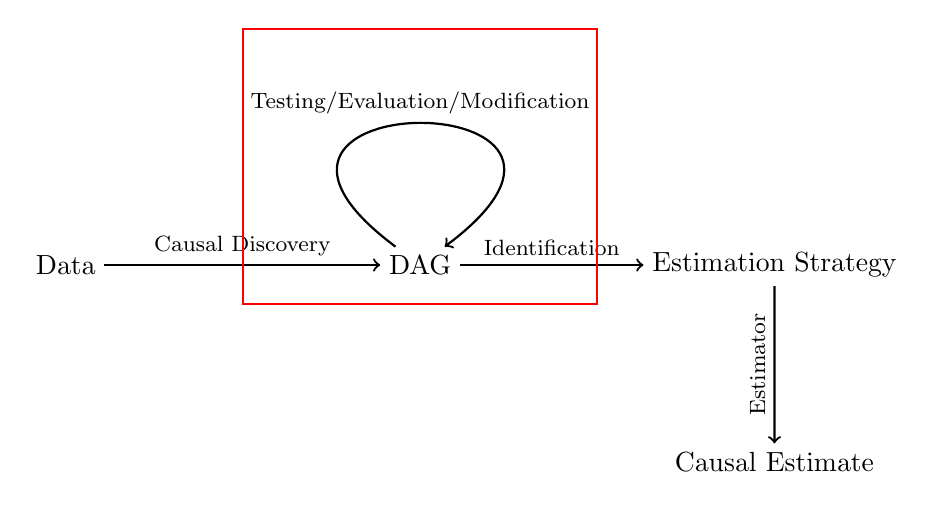
\begin{tikzpicture}[yscale=1, xscale=0.75, inner sep=3pt]
		\tikzstyle{every node}=[align=left]
			\node (data) at (0, 0) {Data};
			\node (dag) at (6, 0) {DAG};
			\node (estimand) at (12, 0) {Estimation Strategy};
			\node (estimation) at (12, -2.5) {Causal Estimate};
	
			\draw[thick, ->] (data) to node[midway, above]{\footnotesize Causal Discovery} (dag);
			\draw[thick, ->] (dag) to node[midway, above] {\footnotesize Identification} (estimand);
			\draw[thick, ->] (estimand) to node[midway, above, rotate=90] {\footnotesize Estimator} (estimation);
			\draw[thick, ->] (dag) [out=150, in=30, looseness=10] to node[midway, above] {\footnotesize Testing/Evaluation/Modification} (dag);

			\draw[draw=red, thick] (3, -0.5) rectangle (9, 3);
		\end{tikzpicture}
		\label{fig:workflow2}
	\end{figure}

	\begin{itemize}
		\item Adding expert knowledge can be helpful, but experts can also make mistakes.
		\item Usually experts end up with very dense models when drawing manually.
	\end{itemize}
\end{frame}

\begin{frame}{Model Evaluation}
	We don't have access to ground truth, so no straight-forward way to evaluate the model.

	\begin{itemize}
		\item Testing implied Conditional Independences (CIs): 
		\item Fisher C: Similar to implied CIs but summerizes the whole model fit.
		\item Data Fit metrics such as likelihood or structure scores to compare models.
	\end{itemize}
\end{frame}

\begin{frame}{Testing Implied Conditional Independences (CIs)}
	\center{Each missing edge in a DAG implies a Conditional Independence (CI) statement.}

	\todo[inline]{Add a figure showing implied CIs}
\end{frame}

\begin{frame}{Testing Implied Conditional Independences (CIs)}
	\begin{enumerate}
		\item A DAG 
		\item Use statistical CI tests to test whether CIs hold in the data.
	\end{enumerate}
\end{frame}

\begin{frame}{Fisher's C and Correlation Score}
	Correlation Score: Scores how well the model structure explains the correlations 
	observed in the data.

	Fisher's C: Combines the CI tests to give a single p-value.
\end{frame}

\begin{frame}{Score metrics}
\end{frame}

\begin{frame}{Causal Discovery Algorithms learn a CPDAG}
	\begin{figure}
	\end{figure}
	
	\begin{itemize}
		\item Trying to learn a network structure which matches the covariance
			structure.
		\item Multiple networks can represent the same casual structure.
		\item Structure learning algorithms usually a DAG.
	\end{itemize}

	Pairwise edge orientation rules.
\end{frame}

\begin{frame}{Minimal Orientation}
\end{frame}

\begin{frame}{LLM Based Causal Discovery}
	\begin{figure}
		\centering
		\includegraphics[scale=0.3]{imgs/adult_llm.png}
	\end{figure}
\end{frame}

% \begin{frame}{Using learned DAG in the PO framework}
% 	As DAGs explicitly show all the information, it can be used to make
% 	decisions in the PO framework as well.
% 
% 	The graph can be put into pywhy as well.
% \end{frame}

\begin{frame}{Identification}
	\begin{figure}
		\centering
		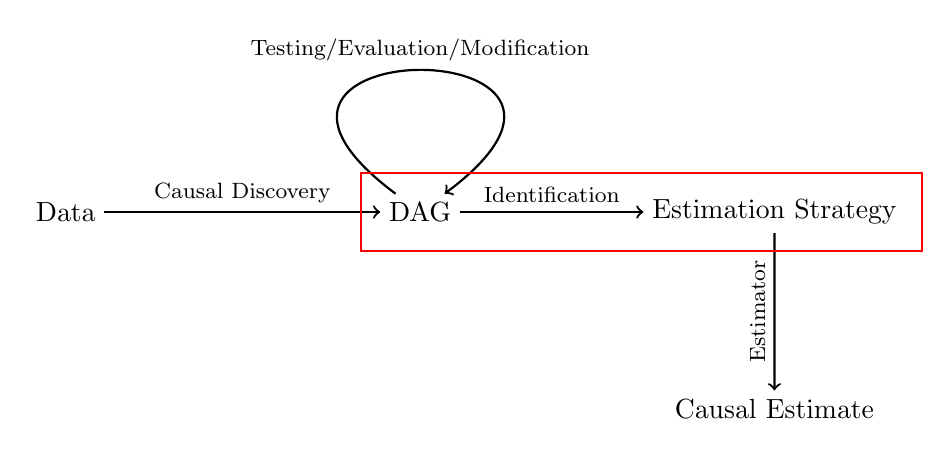
\begin{tikzpicture}[yscale=1, xscale=0.75, inner sep=3pt]
		\tikzstyle{every node}=[align=left]
			\node (data) at (0, 0) {Data};
			\node (dag) at (6, 0) {DAG};
			\node (estimand) at (12, 0) {Estimation Strategy};
			\node (estimation) at (12, -2.5) {Causal Estimate};
	
			\draw[thick, ->] (data) to node[midway, above]{\footnotesize Causal Discovery} (dag);
			\draw[thick, ->] (dag) to node[midway, above] {\footnotesize Identification} (estimand);
			\draw[thick, ->] (estimand) to node[midway, above, rotate=90] {\footnotesize Estimator} (estimation);
			\draw[thick, ->] (dag) [out=150, in=30, looseness=10] to node[midway, above] {\footnotesize Testing/Evaluation/Modification} (dag);

			\draw[draw=red, thick] (5, -0.5) rectangle (14.5, 0.5);
		\end{tikzpicture}
		\label{fig:workflow3}
	\end{figure}
	\begin{itemize}
		\item Once we have decided on the DAG, we can start estimating causal effects.
		\item \textbf{Identification}: Is the causal effect of interest estimable?
		\item Everything is identified if all variables are observed.
	\end{itemize}
\end{frame}

\begin{frame}{do-calculus}
	Theoretically, do-calculus provided a complete solution. 

	\textcolor{red}{However, no efficient algorithms to use it in practice}

	In practice, we use a bunch of simpler identification strategies, each of which
	can identify a subset of effects.

	\todo[inline]{Add a venn diagram here}
\end{frame}

\begin{frame}{Backdoor Criterion}
	\begin{itemize}
		\item Finds adjustment variables to block all confounding paths.
	\end{itemize}
\end{frame}

\begin{frame}{Front-door Criterion}
	\begin{itemize}
		\item Double application of backdoor criterion.
		\item Used for scenarios when there are mediator variables.
	\end{itemize}
\end{frame}

\begin{frame}{Instrumental Variables}
	\begin{itemize}
		\item Use variables which are correlated with the outcome variable only
			through the exposure variable.
	\end{itemize}
\end{frame}

\begin{frame}{Estimation}
	\begin{figure}
		\centering
		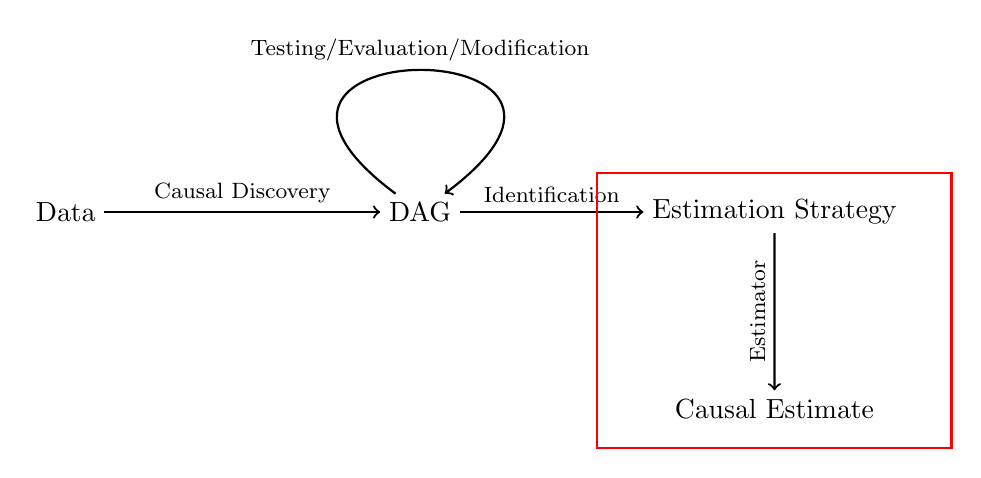
\begin{tikzpicture}[yscale=1, xscale=0.75, inner sep=3pt]
		\tikzstyle{every node}=[align=left]
			\node (data) at (0, 0) {Data};
			\node (dag) at (6, 0) {DAG};
			\node (estimand) at (12, 0) {Estimation Strategy};
			\node (estimation) at (12, -2.5) {Causal Estimate};
	
			\draw[thick, ->] (data) to node[midway, above]{\footnotesize Causal Discovery} (dag);
			\draw[thick, ->] (dag) to node[midway, above] {\footnotesize Identification} (estimand);
			\draw[thick, ->] (estimand) to node[midway, above, rotate=90] {\footnotesize Estimator} (estimation);
			\draw[thick, ->] (dag) [out=150, in=30, looseness=10] to node[midway, above] {\footnotesize Testing/Evaluation/Modification} (dag);

			\draw[draw=red, thick] (9, -3) rectangle (15, 0.5);
		\end{tikzpicture}
		\label{fig:workflow4}
	\end{figure}

	\begin{itemize}
		\item Identification methods give the estimand.
		\item Any estimator can be used to make the estimates.
		\item Usually people use linear models for their interpretability.
		\item pgmpy has a discrete variable inference engine, that can be used
			as well.
	\end{itemize}
\end{frame}

\begin{frame}{Some other functionality}
	\begin{itemize}
		\item Simulations
		\item Extensible
	\end{itemize}
\end{frame}

\begin{frame}{Simulations}

\end{frame}

\begin{frame}{Extensible}
	\begin{itemize}
		\item Very active field of research, lots of new methods are getting developed.
		\item pgmpy offers easy ways to extend/modify algorithms where ever possible.
	\end{itemize}	
	$ random ci_test $
\end{frame}

\begin{frame}{Future Plans}
	\begin{itemize}
		\item Focus on implementing practical methods.
		\item Wider support for mixed data i.e., combination of categorical, ordinal, and continuous variables.
		\item Add few more of the commonly used algorithms.
	\end{itemize}
\end{frame}

\begin{frame}
	\center{\Huge {Thank you}}
	\vspace{5em}

	\github: pgmpy/pgmpy

	\email: ankurankan@gmail.com
\end{frame}

% \begin{frame}{Extra slide}
% 	When to use PO vs DAG framework?
% \end{frame}
% 
% \begin{frame}
% 	How does it compare to Shapley values 
% 	\begin{itemize}
% 		\item Still prediction based. Does not matter if perturbing direct effect variable or undirect.
% 		\item Can show an example where Shapley values would still find an association, but causal inference would not. The standard confounding case.
% 	\end{itemize}
% \end{frame}
\end{document}
